% !TEX root = main.tex

\chapter{Capillary oscillations of a liquid bridge}

\begin{description}
\item{Directory in the StabFem project :}  \texttt{LiquidBridges}
\item{Main contributors :} D. Fabre.
\item{Reference :} Chireux et al., Phys. Fluids, 2015.
\end{description}


\begin{figure}
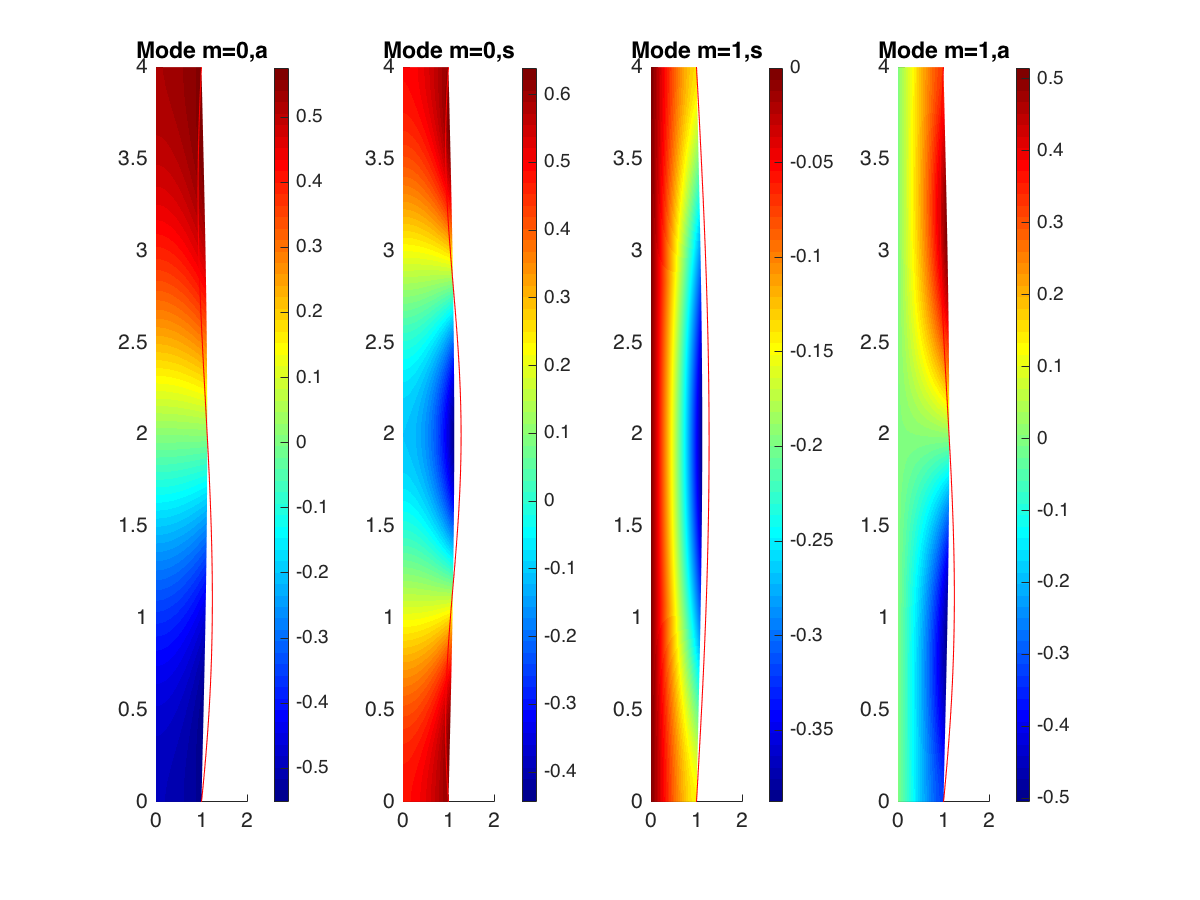
\includegraphics[width=.8\linewidth]{../LiquidBridges/FIGURES/Bridges_NV_Eigenmodes_phi_cyl_L3_5.png}
\caption{Oscillation modes of a liquid bridge of aspect ratio $L/R=4$ and reduced volume $V^ =$...}
\label{Bridges_NV_Eigenmodes_phi_cyl_L3_5}
\end{figure}

\begin{figure}
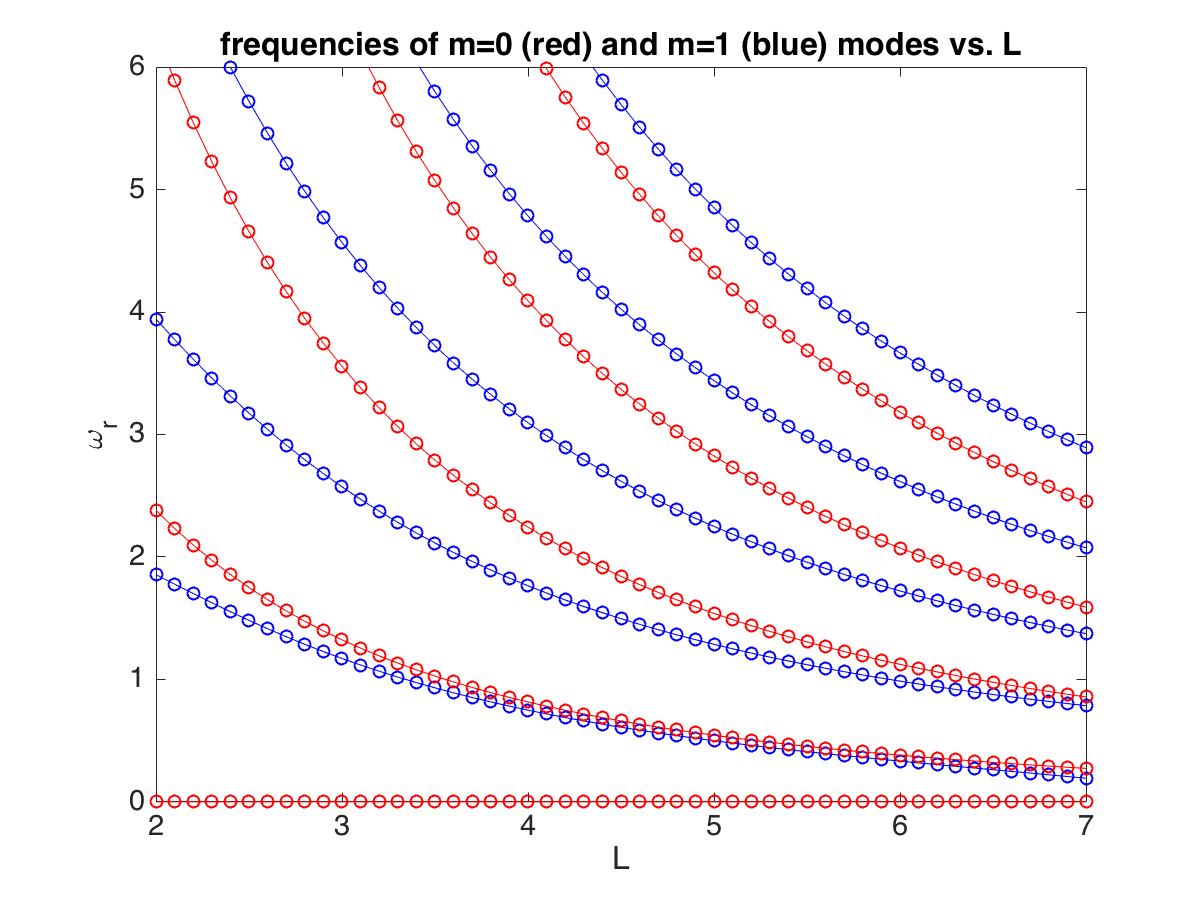
\includegraphics[width=.45\linewidth]{../LiquidBridges/FIGURES/Bridges_NV_coal_omega.png}
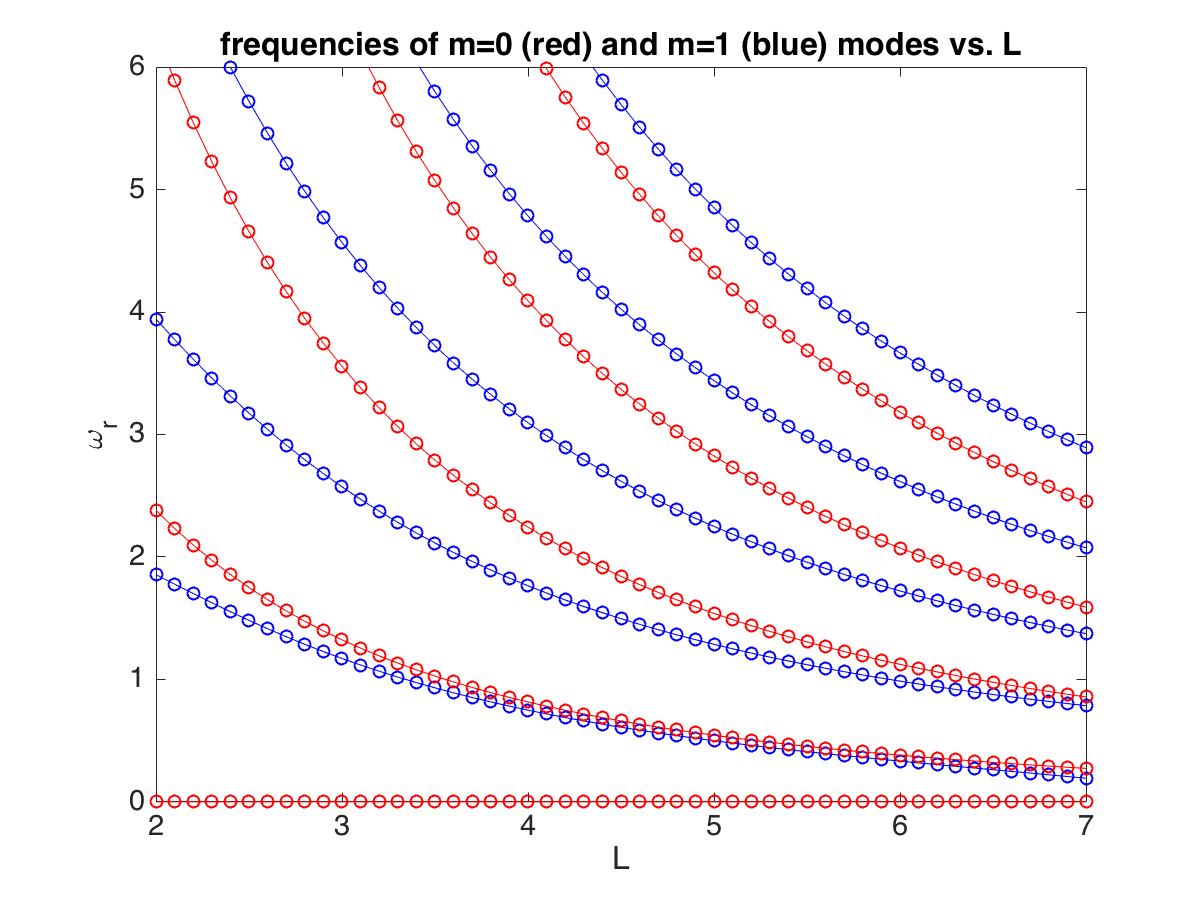
\includegraphics[width=.45\linewidth]{../LiquidBridges/FIGURES/Bridges_NV_coal_omega.png}
\caption{Oscillation frequencies of a liquid bridge resulting from the coalescence of two spherical droplets
as function of $L^* =L/R$
(figures 11,12 of Chireux et al.)
}
\label{Bridges_NV_Eigenmodes_phi_cyl_L3_5}
\end{figure}
 